%=======AOL BEAMER TEMPLATE=======%
%============June 18, 2015============%

\documentclass{article}

%Some packages
\usepackage[margin=0.5in]{geometry}
\usepackage{etex}
\usepackage{hyperref}
\usepackage{natbib}
\usepackage{movie15}
\usepackage{amsmath}
\usepackage{amssymb}
\usepackage{algorithm,algorithmic}
\usepackage{mathtools}
\usepackage{subfigure}
\usepackage{xcolor}
\usepackage{lipsum}
\usepackage{multicol}
\usepackage{multirow}
\usepackage{tcolorbox}
\usepackage{epsfig}
\usepackage{epstopdf}
\usepackage{booktabs}
\usepackage{cancel}
\usepackage{float}
\usepackage{wrapfig}
\usepackage{wrapfig}
\usepackage{tikz}
\definecolor{mag}{rgb}{1, 0, 1}
\usetikzlibrary{shapes.geometric, arrows,fit}
\usetikzlibrary{decorations.pathreplacing,angles,quotes}
\usepackage{tabularx}
\usepackage{hhline}
\usetikzlibrary{patterns}
\usetikzlibrary{calc,through}

\usepackage{pgfplots}
\pgfplotsset{compat=1.12}


\usetikzlibrary{backgrounds}
\tikzset{white background/.style={show background rectangle,tight background, background rectangle/.style={fill=white}}}

\usepgfplotslibrary{external} % creates a tight self-contained pdf figure for each tikzpicture
\tikzexternalize % comment out to debug if latex errors: generates the external pdf
\tikzset{external/force remake} % otherwise will use external pdf if it exists
\tikzset{png export/.style={
	external/system call={
		pdflatex \tikzexternalcheckshellescape
			-halt-on-error -interaction=batchmode -jobname "\image" "\texsource";
		convert -units pixelsperinch -density 150 "\image.pdf" "\image.png";
		convert -units pixelsperinch -density 600 "\image.pdf" "\image-600.png";
}}}
\tikzset{png export}
\tikzsetexternalprefix{figures/} % output the pdf to an existing directory (needs to exist)
\tikzsetnextfilename{myfigure}

\tikzstyle{noBox} = [rectangle, rounded corners, minimum width=2cm, minimum height=1.5cm,text width=3cm, text centered]
\tikzstyle{doublenoBox} = [rectangle, rounded corners, minimum width=2cm, minimum height=1.5cm,text width=6cm, text centered]
\tikzstyle{process} = [rectangle,rounded corners, minimum width=2cm, minimum height=1.cm, text width=3cm, text centered, draw=black,fill=black!10!white]
\tikzstyle{processLong} = [process, text width=3.5cm]
\tikzstyle{dataStack} = [rectangle,rounded corners, minimum width=2cm, minimum height=0.55cm, text width=3cm, text centered, draw=black,fill=black!10!white]
\tikzstyle{arrow} = [line width=0.75mm,->]
\tikzstyle{decision} = [rectangle, rounded corners, minimum height=1.25cm, text width=4cm, text centered, draw=black,fill=black!10!white]


\title{Tikz Figures}
\author{Aaron Babier}
%------------------------------------------------

%Title frame
\begin{document}

\tikzsetnextfilename{ipman-training}
        \begin{figure}
            \centering
            \resizebox{18cm}{!}{%
                        \begin{tikzpicture}[node distance=5cm, white background]
                                \node(topic)[noBox]  {
\includegraphics[width=2cm]{ct.eps}\\ Contoured CT image};
                                \node(defining)[process,right of = topic, yshift=1cm, xshift=3cm] {Generator};
                                \node(collecting)[process,right of = topic,  yshift=-1cm, xshift=5.5cm] {Oracle};
                                \node(applying)[process,right of = topic, yshift=-1cm, xshift=0.5cm] {Classifier};
                                \node(coms)[noBox,right of = topic, xshift=11cm] {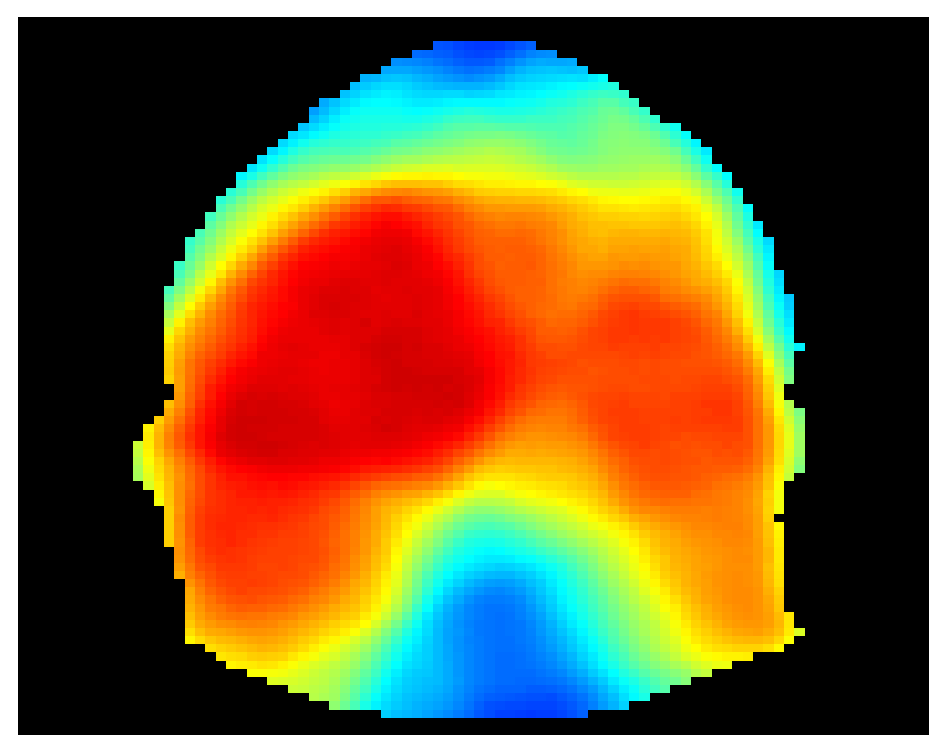
\includegraphics[width=2cm]{dose.eps}\\ Feasible dose};
				% Highlight dose prediction
				\node(cycleHeading)[above of = defining, yshift =-4cm] {\textbf{IPMAN}};
				\node(cyclebottom)[right of = topic, yshift =-2.1cm, xshift=3cm] {\ };
				\node[draw=black,dashed, inner sep=5pt,rounded corners=0.3cm, fit=(cycleHeading)(collecting)(applying)(cyclebottom)]{};
				% Draw arrows
				\draw [arrow, black] ([xshift=0.1cm]topic.east) to ([yshift=1cm, xshift=-0.5cm]applying.west);
				\draw [arrow, black] ([yshift=1cm, xshift=0.5cm]collecting.east) to ([xshift=-0.1cm]coms.west);
				\draw [arrow, black] ([xshift=0.1cm, yshift=-0.1cm]defining.east) to [out=-45, in=100] ([yshift=0.1cm]collecting.north);
				\draw [arrow, black] ([yshift=-0.1cm,  xshift=-1.25cm]collecting.south) to [out=-135, in=-45] ([yshift=-0.10cm, xshift=1.25cm]applying.south);
				\draw [arrow, black] ([yshift=0.1cm]applying.north) to [out=80, in=225] ([xshift=-0.1cm, yshift=-0.1cm]defining.west);
                        \end{tikzpicture}
                }
        \end{figure}
        


\end{document}
